\ifx\pdfminorversion\undefined\else\pdfminorversion=4\fi
\documentclass[aspectratio=169,t,xcolor=dvipsnames]{beamer}
%\documentclass[aspectratio=169,t,handout]{beamer}

% English version FAU Logo
\usepackage[english]{babel}
% German version FAU Logo
%\usepackage[ngerman]{babel}

\usepackage[utf8]{inputenc}
\usepackage[T1]{fontenc}
\usepackage{amsmath,amssymb}
\usepackage{graphicx}
\usepackage{listings}
\usepackage{url}
\usepackage{enumitem}
\usepackage{hyperref}
\usepackage{fontawesome}
\usepackage{graphicx}
\usepackage{booktabs}
\usepackage{calc}
\usepackage{ifthen}
\usepackage{xcolor}
\usepackage{tabularx}
\usepackage{makecell}
\usepackage{tikz}
\usepackage{tikz}
\usepackage{tikz-cd}
\usepackage{verbatim}
\usepackage{pgfplots,pgfplotstable,pgf-pie}
\usepackage{filecontents}
\newcommand{\plots}{0.611201}
\newcommand{\plotm}{2.19882}
\pgfplotsset{height=4cm,width=8cm,compat=1.16}
\pgfmathdeclarefunction{gauss}{2}{%
  \pgfmathparse{1/(#2*sqrt(2*pi))*exp(-((x-#1)^2)/(2*#2^2))}%
}

\tikzset{
    vertex/.style = {
        circle,
        fill            = black,
        outer sep = 2pt,
        inner sep = 1pt,
    }
}

\tikzset{
    mynode/.style={
        draw,
        thick,
        anchor=south west,
        minimum width=2cm,
        minimum height=1.3cm,
        align=center,
        inner sep=0.2cm,
        outer sep=0,
        rectangle split,
        rectangle split parts=2,
        rectangle split draw splits=false},
    reverseclip/.style={
        insert path={(current page.north east) --
            (current page.south east) --
            (current page.south west) --
            (current page.north west) --
            (current page.north east)}
    }
}

\tikzset{basic/.style={
        draw,
        rectangle split,
        rectangle split parts=2,
        rectangle split part fill={blue!20,white},
        minimum width=2.5cm,
        text width=2cm,
        align=left,
        font=\itshape
    },
    Diamond/.style={ diamond,
                      draw,
                      shape aspect=2,
                      inner sep = 2pt,
                      text centered,
                      fill=blue!10!white,
                      font=\itshape
                    }}


\tikzset{level 1/.append style={sibling angle=50,level distance = 165mm}}
\tikzset{level 2/.append style={sibling angle=20,level distance = 45mm}}
\tikzset{every node/.append style={scale=1}}

\usetikzlibrary{arrows,decorations.pathmorphing,backgrounds,fit,positioning,shapes.symbols,chains,intersections,snakes,positioning,matrix,mindmap,shapes.multipart,shapes,calc,shapes.geometric}

% read in data file

\newcommand{\MaxNumberX}{3}
\newcommand{\MaxNumberY}{5}
\newcommand{\tikzmark}[1]{\tikz[remember picture] \node[coordinate] (#1) {#1};}

\pgfplotstableread{data/iris.dat}\iris
\pgfplotstablegetrowsof{\iris}
\pgfplotsset{compat=1.14}
\pgfmathsetmacro\NumRows{\pgfplotsretval-1}
\definecolor{airforceblue}{rgb}{0.36, 0.54, 0.66}

\usepgfplotslibrary{groupplots}
% Options:
%  - inst:      Institute
%                 med:      MedFak FAU theme
%                 nat:      NatFak FAU theme
%                 phil:     PhilFak FAU theme
%                 rw:       RWFak FAU theme
%                 rw-jura:  RWFak FB Jura FAU theme
%                 rw-wiso:  RWFak FB WISO FAU theme
%                 tf:       TechFak FAU theme
%  - image:     Cover image on title page
%  - plain:     Plain title page
%  - longtitle: Title page layout for long title
\usetheme[%
  image,%
  longtitle,%
  tf
]{fau}

% Enable semi-transparent animation preview
\setbeamercovered{transparent}

\lstset{%
  language=Python,
  tabsize=2,
  basicstyle=\tt,
  keywordstyle=\color{blue},
  commentstyle=\color{green!50!black},
  stringstyle=\color{red},
  numbers=left,
  numbersep=0.5em,
  xleftmargin=1em,
  numberstyle=\tt
}
\newcommand{\blue}[1]{\textbf{\textcolor{blue}{#1}}}
% Title, authors, and date
\title[KDD]{Chapter VII: Cluster analysis}
\subtitle{Knowledge Discovery in Databases}
\author[L.~Melodia]{Luciano Melodia M.A.}
% English version
\institute[Department]{Evolutionary Data Management, Friedrich-Alexander University Erlangen-Nürnberg}
% German version
%\institute[Lehrstuhl]{Lehrstuhl, Friedrich-Alexander-Universit\"at Erlangen-N\"urnberg}
\date{Summer semester 2021}
% Set additional logo (overwrites FAU seal)
%\logo{\includegraphics[width=.15\textwidth]{themefau/art/xxx/xxx.pdf}}
\begin{document}
\tikzset{
  every overlay node/.style={
    rounded corners,anchor=north west,
  },
}
% Usage:
% \tikzoverlay at (-1cm,-5cm) {content};
% or
% \tikzoverlay[text width=5cm] at (-1cm,-5cm) {content};
\def\tikzoverlay{%
   \tikz[baseline,overlay]\node[every overlay node]
}%

  % Title
  \maketitle
{  \setbeamertemplate{footline}[frame number]  
\begin{frame}
	\frametitle{Chapter 8: Outlier Analysis}
	\begin{itemize}
		\item \alert{Outlier and Outlier Analysis}
		\item Outlier-Detection Methods
		\item Statistical Approaches
		\item Proximity-Based Approaches
		\item Summary
	\end{itemize}
\end{frame}
}
  
{  \setbeamertemplate{footline}[frame number]
\begin{frame}
   \frametitle{What are Outliers?}
   \begin{itemize}
   	\item \alert{Outlier}:
   	\begin{itemize}
   		\item A data object that \blue{deviates significantly} from the normal objects as if it were generated by a different mechanism
 		\begin{itemize}
 			\item Ex.: unusual credit card purchase,\\
 			sports: Michael Jordon, Wayne Gretzky, ...
 		\end{itemize}
   	\end{itemize}
   	
	\item \textbf{Outliers are different from noise.}
		\begin{itemize}
			\item Noise is a random error or variance in a measured variable.
			\item Noise should be removed before outlier detection.	
		\end{itemize}

	\item \textbf{Outliers are interesting.}
		\begin{itemize}
			\item They violate the mechanism that generates the normal data.
		\end{itemize}
	\item \textbf{Outlier detection vs. novelty detection:}
		\begin{itemize}
			\item Early stage: outlier; but later merged into the model
   		\end{itemize}
   \end{itemize}
\end{frame}
}

%

\begin{frame}
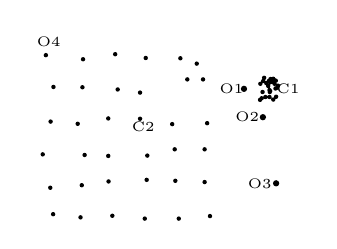
\begin{tikzpicture}[thick,scale=0.4, every node/.style={scale=5}]
\fill (0.14, 0.02)  circle (0.7mm) (0.05, 0.86)  circle (0.7mm) (-0.19, 1.92)  circle (0.7mm) (0.06, 2.96)  circle (0.7mm) (0.15, 4.06)  circle (0.7mm) (-0.09, 5.07)  circle (0.7mm) (1.01, -0.08)  circle (0.7mm) (1.05, 0.94)  circle (0.7mm) (1.14, 1.9)  circle (0.7mm) (0.92, 2.89)  circle (0.7mm) (1.07, 4.05)  circle (0.7mm) (1.09, 4.94)  circle (0.7mm) (2.02, -0.03)  circle (0.7mm) (1.9, 1.06)  circle (0.7mm) (1.89, 1.87)  circle (0.7mm) (1.89, 3.06)  circle (0.7mm) (2.19, 3.98)  circle (0.7mm) (2.11, 5.1)  circle (0.7mm) (3.05, -0.12)  circle (0.7mm) (3.11, 1.11)  circle (0.7mm) (3.13, 1.88)  circle (0.7mm) (2.9, 3.05)  circle (0.7mm) (2.9, 3.88)  circle (0.7mm) (3.08, 4.98)  circle (0.7mm) (4.13, -0.12)  circle (0.7mm) (4.02, 1.08)  circle (0.7mm) (4.0, 2.08)  circle (0.7mm) (3.92, 2.88)  circle (0.7mm) (4.4, 4.3)  circle (0.7mm) (4.18, 4.97)  circle (0.7mm) (5.12, -0.04)  circle (0.7mm) (4.95, 1.04)  circle (0.7mm) (4.95, 2.08)  circle (0.7mm) (5.03, 2.91)  circle (0.7mm) (4.9, 4.3)  circle (0.7mm) (4.7, 4.8)  circle (0.7mm) ; 

%cluster
\fill (7.22, 4.02)  circle (0.7mm) (7.01, 3.74)  circle (0.7mm) (7.17, 4.16)  circle (0.7mm) (7.04, 4.31)  circle (0.7mm) (7.28, 4.1)  circle (0.7mm) (7.22, 3.75)  circle (0.7mm) (6.99, 4.25)  circle (0.7mm) (7.13, 3.66)  circle (0.7mm) (7.03, 3.93)  circle (0.7mm) (6.84, 4.35)  circle (0.7mm) (6.72, 4.16)  circle (0.7mm) (7.14, 4.27)  circle (0.7mm) (6.88, 3.74)  circle (0.7mm) (7.04, 4.21)  circle (0.7mm) (6.79, 3.9)  circle (0.7mm) (7.01, 3.96)  circle (0.7mm) (7.13, 4.32)  circle (0.7mm) (6.71, 3.65)  circle (0.7mm) (6.76, 3.7)  circle (0.7mm) (7.21, 4.26)  circle (0.7mm) (7.02, 3.9)  circle (0.7mm) (7.2, 4.01)  circle (0.7mm) (6.91, 4.18)  circle (0.7mm) (6.81, 4.25)  circle (0.7mm) (6.97, 4.09)  circle (0.7mm);

%outlier O3
\fill (7.22, 1)  circle (1mm);
\node[scale = 0.2] at (6.7, 1)    {\tiny O3};

%O1
\fill (6.2, 4)  circle (1mm);
\node[scale = 0.2] at (5.8, 4)    {\tiny O1};

%O2
\fill (6.8, 3.1)  circle (1mm);
\node[scale = 0.2] at (6.3, 3.1)    {\tiny O2};


\node[scale = 0.2] at (7.6, 4)    {\tiny C1};
\node[scale = 0.2] at (3, 2.8)    {\tiny C2};
\node[scale = 0.2] at (0, 5.5)    {\tiny O4};
\end{tikzpicture}
\tikzoverlay at (12cm,0.60cm) {
	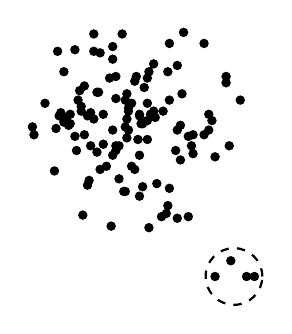
\begin{tikzpicture}[thick,scale=2, every node/.style={scale=5}]
\fill (1.21, 0.56)  circle (0.3mm) (0.51, 1.02)  circle (0.3mm) (0.61, 1.44)  circle (0.3mm) (0.91, 1.54)  circle (0.3mm) (0.69, 0.58)  circle (0.3mm) (1.2, 1.3)  circle (0.3mm) (1.28, 0.96)  circle (0.3mm) (0.67, 1.21)  circle (0.3mm) (0.34, 0.95)  circle (0.3mm) (0.89, 0.83)  circle (0.3mm) (1.33, 0.38)  circle (0.3mm) (1.3, 1.55)  circle (0.3mm) (1.07, 0.99)  circle (0.3mm) (0.89, 0.62)  circle (0.3mm) (1.07, 0.87)  circle (0.3mm) (0.48, 0.67)  circle (0.3mm) (0.35, 0.9)  circle (0.3mm) (1.26, 1.34)  circle (0.3mm) (0.73, 1.54)  circle (0.3mm) (0.76, 1.17)  circle (0.3mm) (1.02, 1.03)  circle (0.3mm) (1.28, 0.74)  circle (0.3mm) (0.54, 1.3)  circle (0.3mm) (0.73, 1.43)  circle (0.3mm) (0.77, 1.42)  circle (0.3mm) (0.85, 0.93)  circle (0.3mm) (0.97, 1.1)  circle (0.3mm) (1.08, 1.3)  circle (0.3mm) (0.5, 1.43)  circle (0.3mm) (1.25, 0.8)  circle (0.3mm) (1.59, 0.83)  circle (0.3mm) (1.02, 0.51)  circle (0.3mm) (0.79, 0.84)  circle (0.3mm) (1.11, 1.05)  circle (0.3mm) (1.2, 0.45)  circle (0.3mm) (1.66, 1.12)  circle (0.3mm) (0.66, 0.39)  circle (0.3mm) (1.57, 1.27)  circle (0.3mm) (1.19, 0.4)  circle (0.3mm) (0.84, 0.32)  circle (0.3mm) (1.36, 0.9)  circle (0.3mm) (1.21, 1.48)  circle (0.3mm) (1.04, 0.57)  circle (0.3mm) (0.87, 0.83)  circle (0.3mm) (0.92, 0.54)  circle (0.3mm) (0.85, 1.46)  circle (0.3mm) (1.16, 0.38)  circle (0.3mm) (0.94, 0.88)  circle (0.3mm) (1.13, 0.59)  circle (0.3mm) (0.71, 0.83)  circle (0.3mm) (1.26, 0.37)  circle (0.3mm) (1.07, 0.87)  circle (0.3mm) (1.57, 1.23)  circle (0.3mm) (0.62, 0.8)  circle (0.3mm) (1.5, 0.76)  circle (0.3mm) (0.42, 1.1)  circle (0.3mm) (1.43, 1.48)  circle (0.3mm) (1.43, 0.9)  circle (0.3mm) (0.49, 0.94)  circle (0.3mm) (1.08, 0.31)  circle (0.3mm) 

(1.04, 0.97)  circle (0.3mm) (0.95, 0.93)  circle (0.3mm) (1.05, 1.2)  circle (0.3mm) (0.54, 0.98)  circle (0.3mm) (0.71, 1.04)  circle (0.3mm) (0.75, 1.17)  circle (0.3mm) (1.07, 1.26)  circle (0.3mm) (0.63, 1.12)  circle (0.3mm) (0.65, 1.08)  circle (0.3mm) (0.95, 1.05)  circle (0.3mm) (0.83, 1.26)  circle (0.3mm) (0.77, 0.68)  circle (0.3mm) (1.02, 0.77)  circle (0.3mm) (0.64, 1.18)  circle (0.3mm) (0.99, 0.68)  circle (0.3mm) (1.21, 1.12)  circle (0.3mm) (0.75, 0.79)  circle (0.3mm) (1.17, 1.05)  circle (0.3mm) (1.01, 0.87)  circle (0.3mm) (0.69, 1.02)  circle (0.3mm) (1.46, 0.93)  circle (0.3mm) (1.02, 1.02)  circle (0.3mm) (1.26, 0.93)  circle (0.3mm) (1.12, 1.01)  circle (0.3mm) (1.46, 1.03)  circle (0.3mm) (0.93, 0.95)  circle (0.3mm) (0.67, 0.9)  circle (0.3mm) (1.0, 1.27)  circle (0.3mm) (0.99, 1.24)  circle (0.3mm) (0.81, 0.7)  circle (0.3mm) (0.93, 0.54)  circle (0.3mm) (0.97, 0.7)  circle (0.3mm) (0.57, 0.96)  circle (0.3mm) (0.55, 1.01)  circle (0.3mm) (1.33, 0.89)  circle (0.3mm) (0.87, 0.8)  circle (0.3mm) (1.11, 1.35)  circle (0.3mm) (0.85, 1.38)  circle (0.3mm) (0.52, 1.04)  circle (0.3mm) (0.7, 0.61)  circle (0.3mm) (1.48, 0.99)  circle (0.3mm) (1.03, 0.97)  circle (0.3mm) (1.07, 1.1)  circle (0.3mm) (0.65, 1.05)  circle (0.3mm) (0.73, 1.0)  circle (0.3mm) (0.87, 1.13)  circle (0.3mm) (0.87, 1.27)  circle (0.3mm) (1.29, 1.16)  circle (0.3mm) (0.79, 1.03)  circle (0.3mm) (0.94, 1.0)  circle (0.3mm) (0.61, 0.89)  circle (0.3mm) (1.35, 0.83)  circle (0.3mm) (1.36, 0.78)  circle (0.3mm) (0.94, 1.16)  circle (0.3mm) (1.09, 1.03)  circle (0.3mm) (0.85, 0.77)  circle (0.3mm) (0.58, 1.03)  circle (0.3mm) (0.95, 1.07)  circle (0.3mm) (0.58, 0.97)  circle (0.3mm) (0.93, 1.12)  circle (0.3mm);


\draw[dashed] (1.62,0) circle (1.8mm); 
\fill (1.7,0)  circle (0.3mm) (1.75,0)  circle (0.3mm) (1.5,0)  circle (0.3mm) (1.6,0.1)  circle (0.3mm);

\end{tikzpicture}};


\end{frame}





{
    \setbeamertemplate{footline}[frame number]
\begin{frame}
  \frametitle{Outliers (2)}
  \begin{itemize}
    \item \textbf{Applications}:
          \begin{itemize}
            \item Credit-card-fraud detection
            \item Telecom-fraud detection
            \item Customer segmentation
            \item Medical analysis
          \end{itemize}
  \end{itemize}
\end{frame}
}

%

{
    \setbeamertemplate{footline}[frame number]
  \begin{frame}
   \frametitle{Types of Outliers}
	\begin{itemize}
	\item Three kinds: global, contextual, and collective outliers
	 \item \alert{Global} outlier (or \blue{point anomaly}):
    	\begin{itemize}
    	    \item Significantly deviates from the rest of the data set
    	    \begin{itemize}
    	        \item Ex.: intrusion detection in computer networks
    	    \end{itemize}
    	    \item Issue: Find an appropriate measurement of deviation
    	\end{itemize}
    \item \alert{Contextual} outlier (or conditional outlier):
        \begin{itemize}
            \item Deviates significantly based on a selected context
                \begin{itemize}
                    \item Ex.:  $80^{\circ}$F in Urbana outlier? (depending on summer or winter)
                \end{itemize}
            \item Attributes of data objects divided into two groups:
                \begin{itemize}
                    \item \textbf{Contextual attributes}: define the context, e.g., time \& location 
                    \item \textbf{Behavioral attributes}: characteristics of the object, used in outlier evaluation, e.g., temperature
                \end{itemize}
            \item Can be viewed as a generalization of local outliers - whose density significantly deviates from its local area
            \item Issue: How to define or formulate meaningful context?
        \end{itemize}
	\end{itemize}
	
	\tikzoverlay at (12cm,7cm) {
	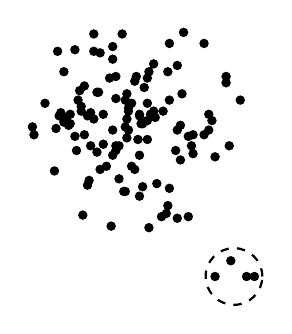
\begin{tikzpicture}[thick,scale=2, every node/.style={scale=5}]
	\fill (1.21, 0.56)  circle (0.3mm) (0.51, 1.02)  circle (0.3mm) (0.61, 1.44)  circle (0.3mm) (0.91, 1.54)  circle (0.3mm) (0.69, 0.58)  circle (0.3mm) (1.2, 1.3)  circle (0.3mm) (1.28, 0.96)  circle (0.3mm) (0.67, 1.21)  circle (0.3mm) (0.34, 0.95)  circle (0.3mm) (0.89, 0.83)  circle (0.3mm) (1.33, 0.38)  circle (0.3mm) (1.3, 1.55)  circle (0.3mm) (1.07, 0.99)  circle (0.3mm) (0.89, 0.62)  circle (0.3mm) (1.07, 0.87)  circle (0.3mm) (0.48, 0.67)  circle (0.3mm) (0.35, 0.9)  circle (0.3mm) (1.26, 1.34)  circle (0.3mm) (0.73, 1.54)  circle (0.3mm) (0.76, 1.17)  circle (0.3mm) (1.02, 1.03)  circle (0.3mm) (1.28, 0.74)  circle (0.3mm) (0.54, 1.3)  circle (0.3mm) (0.73, 1.43)  circle (0.3mm) (0.77, 1.42)  circle (0.3mm) (0.85, 0.93)  circle (0.3mm) (0.97, 1.1)  circle (0.3mm) (1.08, 1.3)  circle (0.3mm) (0.5, 1.43)  circle (0.3mm) (1.25, 0.8)  circle (0.3mm) (1.59, 0.83)  circle (0.3mm) (1.02, 0.51)  circle (0.3mm) (0.79, 0.84)  circle (0.3mm) (1.11, 1.05)  circle (0.3mm) (1.2, 0.45)  circle (0.3mm) (1.66, 1.12)  circle (0.3mm) (0.66, 0.39)  circle (0.3mm) (1.57, 1.27)  circle (0.3mm) (1.19, 0.4)  circle (0.3mm) (0.84, 0.32)  circle (0.3mm) (1.36, 0.9)  circle (0.3mm) (1.21, 1.48)  circle (0.3mm) (1.04, 0.57)  circle (0.3mm) (0.87, 0.83)  circle (0.3mm) (0.92, 0.54)  circle (0.3mm) (0.85, 1.46)  circle (0.3mm) (1.16, 0.38)  circle (0.3mm) (0.94, 0.88)  circle (0.3mm) (1.13, 0.59)  circle (0.3mm) (0.71, 0.83)  circle (0.3mm) (1.26, 0.37)  circle (0.3mm) (1.07, 0.87)  circle (0.3mm) (1.57, 1.23)  circle (0.3mm) (0.62, 0.8)  circle (0.3mm) (1.5, 0.76)  circle (0.3mm) (0.42, 1.1)  circle (0.3mm) (1.43, 1.48)  circle (0.3mm) (1.43, 0.9)  circle (0.3mm) (0.49, 0.94)  circle (0.3mm) (1.08, 0.31)  circle (0.3mm) 

(1.04, 0.97)  circle (0.3mm) (0.95, 0.93)  circle (0.3mm) (1.05, 1.2)  circle (0.3mm) (0.54, 0.98)  circle (0.3mm) (0.71, 1.04)  circle (0.3mm) (0.75, 1.17)  circle (0.3mm) (1.07, 1.26)  circle (0.3mm) (0.63, 1.12)  circle (0.3mm) (0.65, 1.08)  circle (0.3mm) (0.95, 1.05)  circle (0.3mm) (0.83, 1.26)  circle (0.3mm) (0.77, 0.68)  circle (0.3mm) (1.02, 0.77)  circle (0.3mm) (0.64, 1.18)  circle (0.3mm) (0.99, 0.68)  circle (0.3mm) (1.21, 1.12)  circle (0.3mm) (0.75, 0.79)  circle (0.3mm) (1.17, 1.05)  circle (0.3mm) (1.01, 0.87)  circle (0.3mm) (0.69, 1.02)  circle (0.3mm) (1.46, 0.93)  circle (0.3mm) (1.02, 1.02)  circle (0.3mm) (1.26, 0.93)  circle (0.3mm) (1.12, 1.01)  circle (0.3mm) (1.46, 1.03)  circle (0.3mm) (0.93, 0.95)  circle (0.3mm) (0.67, 0.9)  circle (0.3mm) (1.0, 1.27)  circle (0.3mm) (0.99, 1.24)  circle (0.3mm) (0.81, 0.7)  circle (0.3mm) (0.93, 0.54)  circle (0.3mm) (0.97, 0.7)  circle (0.3mm) (0.57, 0.96)  circle (0.3mm) (0.55, 1.01)  circle (0.3mm) (1.33, 0.89)  circle (0.3mm) (0.87, 0.8)  circle (0.3mm) (1.11, 1.35)  circle (0.3mm) (0.85, 1.38)  circle (0.3mm) (0.52, 1.04)  circle (0.3mm) (0.7, 0.61)  circle (0.3mm) (1.48, 0.99)  circle (0.3mm) (1.03, 0.97)  circle (0.3mm) (1.07, 1.1)  circle (0.3mm) (0.65, 1.05)  circle (0.3mm) (0.73, 1.0)  circle (0.3mm) (0.87, 1.13)  circle (0.3mm) (0.87, 1.27)  circle (0.3mm) (1.29, 1.16)  circle (0.3mm) (0.79, 1.03)  circle (0.3mm) (0.94, 1.0)  circle (0.3mm) (0.61, 0.89)  circle (0.3mm) (1.35, 0.83)  circle (0.3mm) (1.36, 0.78)  circle (0.3mm) (0.94, 1.16)  circle (0.3mm) (1.09, 1.03)  circle (0.3mm) (0.85, 0.77)  circle (0.3mm) (0.58, 1.03)  circle (0.3mm) (0.95, 1.07)  circle (0.3mm) (0.58, 0.97)  circle (0.3mm) (0.93, 1.12)  circle (0.3mm);


\draw[dashed] (1.62,0) circle (1.8mm); 
\fill (1.7,0)  circle (0.3mm) (1.75,0)  circle (0.3mm) (1.5,0)  circle (0.3mm) (1.6,0.1)  circle (0.3mm);

\end{tikzpicture}};
	
	
\end{frame}
}

%

{
\setbeamertemplate{footline}[frame number]
\begin{frame}
	\frametitle{Types of Outliers(2)}
	\begin{itemize}
	\item \alert{Collective} \textbf{Outlier}:
	\begin{itemize}
	    \item A \textbf{subset} of data Objects that collectively deviates significantly from the\\ whole data set %what is significantly?
	    \item Ex.: intrusion detection - A number of computers keep sending\\ denial-of-service packages to each other.
	\end{itemize}
	
	\item \textbf{Detection of collective outliers}
		\begin{itemize}
			\item Consider not only behavior of individual objects,but also that of groups of objects
			\item Need to have the background knowledge on the relationship among data objects, such as a distance or similarity measure on objects
		\end{itemize}
	\item \textbf{A data set may have multiple types of outliers.}
	\item \textbf{One object may belong to more than one type of outlier.}

	\end{itemize}
	\tikzoverlay at (12cm,6cm) {
	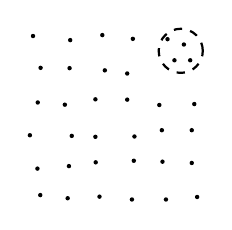
\begin{tikzpicture}[thick,scale=0.4, every node/.style={scale=5}]
	\fill (0.14, 0.02)  circle (0.7mm) (0.05, 0.86)  circle (0.7mm) (-0.19, 1.92)  circle (0.7mm) (0.06, 2.96)  circle (0.7mm) (0.15, 4.06)  circle (0.7mm) (-0.09, 5.07)  circle (0.7mm) (1.01, -0.08)  circle (0.7mm) (1.05, 0.94)  circle (0.7mm) (1.14, 1.9)  circle (0.7mm) (0.92, 2.89)  circle (0.7mm) (1.07, 4.05)  circle (0.7mm) (1.09, 4.94)  circle (0.7mm) (2.02, -0.03)  circle (0.7mm) (1.9, 1.06)  circle (0.7mm) (1.89, 1.87)  circle (0.7mm) (1.89, 3.06)  circle (0.7mm) (2.19, 3.98)  circle 	(0.7mm) (2.11, 5.1)  circle (0.7mm) (3.05, -0.12)  circle (0.7mm) (3.11, 1.11)  circle (0.7mm) (3.13, 1.88)  circle (0.7mm) (2.9, 3.05)  circle (0.7mm) (2.9, 3.88)  circle (0.7mm) (3.08, 4.98)  circle (0.7mm) (4.13, -0.12)  circle (0.7mm) (4.02, 1.08)  circle (0.7mm) (4.0, 2.08)  circle (0.7mm) (3.92, 2.88)  circle (0.7mm) (4.4, 4.3)  circle (0.7mm) (4.18, 4.97)  circle (0.7mm) (5.12, -0.04)  circle (0.7mm) (4.95, 1.04)  circle (0.7mm) (4.95, 2.08)  circle (0.7mm) (5.03, 2.91)  circle (0.7mm) (4.9, 4.3)  circle (0.7mm) (4.7, 4.8)  circle (0.7mm) ; 
	\draw[dashed] (4.6,4.6) circle (7mm);

	\end{tikzpicture}};	
\end{frame} 
}

%

\begin{frame}{Challenges of Outlier Detection}
\begin{itemize}
    \item \textbf{Modeling normal objects and outliers properly}
    \begin{itemize}
        \item Hard to enumerate all possible normal behaviors in an application
        \item The border between normal and outlier objects is often a grey area.
    \end{itemize}
    \item \textbf{Application-specific outlier detection}
    \begin{itemize}
        \item Choice of distance measure among objects and the model of relationship among objects are application-dependent.
        \item E.g. clinical data: a small deviation could be an outlier; while in marketing analysis: larger fluctuations
    \end{itemize}
    \item \textbf{Handling noise in outlier detection}
    \begin{itemize}
        \item Noise may distort the normal objects and blur the distinction between normal objects and outliers.
        \item It may hide outliers and reduce the effectiveness of outlier detection.
    \end{itemize}
    \item \textbf{Understandability}
    \begin{itemize}
        \item Understand why these are outliers: justification of the detection
        \item Specify the degree of an outlier: the unlikelihood of the object being generated by a normal mechanism
    \end{itemize}
\end{itemize}    
\end{frame}

%

\begin{frame}{Chapter: 8 Outlier Analysis}
\bf
    \begin{itemize}
        \item Outlier and Outlier Analysis
        \item \alert{ Outlier-Detection Methods}
        \item Statistical Approaches
        \item Proximity-Based Approaches
        \item Summary
    \end{itemize}
\end{frame}

%

\begin{frame}{Outlier Detection I: Supervised Methods}
    \begin{itemize}
        \item \textbf{Two ways to categorize outlier-detection methods:} 
        \begin{itemize}
            \item Based on whether \blue{user-labeled examples of outliers} can be obtained:\\ \qquad 
            Supervised, semi-supervised vs. unsupervised methods
            \item Based on assumptions about normal data and outliers:\\ \qquad
            Statistical, proximity-based, and clustering-based methods
        
        \end{itemize}
        \item \textbf{Outlier Detection I: Supervised Methods}
  
        \begin{itemize}
            \item Modeling outlier detection as a \blue{classification problem}:\\ \qquad
            Samples examined by domain experts used for training \& testing
            \item Methods for learning a classifier for outlier detection effectively:
            \begin{itemize}
            \item Model normal objects \& report those not matching the model as outliers, or
            \item Model outliers and treat those not matching the model as normal 
            \end{itemize}
            \item Challenges
            \begin{itemize}
                \item Imbalanced classes, i.e., outliers are rare: \\ \qquad Boost the outlier class and make up some artificial outliers
                \item Catch as many outliers as possible, i.e., recall is more important than accuracy (i.e., not mislabeling normal objects as outliers)
                \end{itemize}
            \end{itemize}
    \end{itemize}
\end{frame}

%

\begin{frame}
	\frametitle{Outlier Detection II: Unsupervised Methods }
	\begin{itemize}
		\item \textbf{Assume the \blue{normal objects are somewhat "clustered"} into multiple groups, each having some distinct features.}
		\item\textbf{ An outlier is expected to be \blue{far away from any group} of normal objects.}
		\item \textbf{Weakness: Cannot detect collective outliers effectively}
		      \begin{itemize}
		      	\item Normal objects may not share any strong pattern, but the collective outliers may have high similarity in a small area.
		      \end{itemize}
		\item \textbf{Ex.: In some intrusion or virus detection, normal activities are diverse.}
		      \begin{itemize}
		      	\item Unsupervised methods may have a high false-positive rate, but still miss many real outliers.
		      	\item Supervised methods can be more effective, e.g., identify attacking some key resources.
		      \end{itemize}
		\item \textbf{Many clustering methods can be adapted for unsupervised methods.}
		      \begin{itemize}
		      	\item Find clusters, then outliers: not belonging to any cluster
		      	\item Problem 1: Hard to distinguish noise from outliers
		      	\item Problem 2: Costly since first clustering, but far less outliers than normal objects
		      	      \begin{itemize}
		      	      	\item Newer methods: tackle outliers directly
		      	      \end{itemize}
		      \end{itemize}
	\end{itemize}
\end{frame}

%

\begin{frame}
	\frametitle{Outlier Detection III: Semi-Supervised Methods }
	\begin{itemize}
		\item \textbf{Situation:}
		      \begin{itemize}
		      	\item In many applications, the \blue{number of labeled data objects is small}:Labels could be on outliers only, on normal objects only, or on both.
		      \end{itemize}
		\item \textbf{Semi-supervised outlier detection}
		      \begin{itemize}
		      	\item Regarded as application of semi-supervised learning
		      \end{itemize}
		\item \textbf{If some \blue{labeled normal objects} are available:}
		      \begin{itemize}
		      	\item Use the labeled examples and the proximate unlabeled objectsto train a model for normal objects.
		      	\item Those not fitting the model of normal objects are detected as outliers.
		      \end{itemize}
		\item \textbf{If only some \blue{labeled outliers} are available,that small number may not cover the possible outliers well.}
		      \begin{itemize}
		      	\item To improve the quality of outlier detection:get help from models for normal objects learned from unsupervised methods.
		      \end{itemize}
	\end{itemize}
\end{frame}

%

\begin{frame}
	\frametitle{Outlier Detection (1): Statistical Methods}
	\begin{itemize}
		\item (Also known as model-based methods)
		\item Assume that the \blue{normal data follow some statistical model}.
		      \begin{itemize}
		      	\item The data not following the model are outliers.
		      \end{itemize}
		\item \textbf{Example (right figure):}
		      \begin{itemize}
		      	\item First use Gaussian distribution \alert{$g_D$} to model the normal data.
		      	\item For each object \alert{$y$} in region \alert{$R$}, estimate $g_D(y)$, the probability that $y$ fits\\ the Gaussian distribution
		      	\item If $g_D(y)$ is very low, $y$ is unlikely generated by the Gaussian model, thus an outlier.
		      \end{itemize}
		\item\textbf{ Effectiveness of statistical methods}
		      \begin{itemize}
		      	\item Highly depends on whether the assumption of statistical model holds in the real data
		      \end{itemize}
		\item \textbf{There are many kinds of statistical models.}
		      \begin{itemize}
		      	\item E.g., parametric vs. non-parametric
		      \end{itemize}
	\end{itemize}
	
	\tikzoverlay at (12cm,7cm) {
	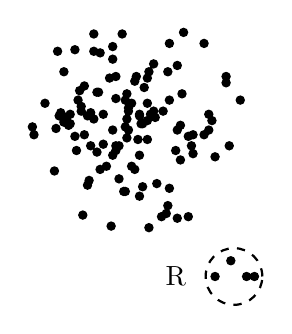
\begin{tikzpicture}[thick,scale=2, every node/.style={scale=5}]
	\fill (1.21, 0.56)  circle (0.3mm) (0.51, 1.02)  circle (0.3mm) (0.61, 1.44)  circle (0.3mm) (0.91, 1.54)  circle (0.3mm) (0.69, 0.58)  circle (0.3mm) (1.2, 1.3)  circle (0.3mm) (1.28, 0.96)  circle (0.3mm) (0.67, 1.21)  circle (0.3mm) (0.34, 0.95)  circle (0.3mm) (0.89, 0.83)  circle (0.3mm) (1.33, 0.38)  circle (0.3mm) (1.3, 1.55)  circle (0.3mm) (1.07, 0.99)  circle (0.3mm) (0.89, 0.62)  circle (0.3mm) (1.07, 0.87)  circle (0.3mm) (0.48, 0.67)  circle (0.3mm) (0.35, 0.9)  circle (0.3mm) (1.26, 1.34)  circle (0.3mm) (0.73, 1.54)  circle (0.3mm) (0.76, 1.17)  circle (0.3mm) (1.02, 1.03)  circle (0.3mm) (1.28, 0.74)  circle (0.3mm) (0.54, 1.3)  circle (0.3mm) (0.73, 1.43)  circle (0.3mm) (0.77, 1.42)  circle (0.3mm) (0.85, 0.93)  circle (0.3mm) (0.97, 1.1)  circle (0.3mm) (1.08, 1.3)  circle (0.3mm) (0.5, 1.43)  circle (0.3mm) (1.25, 0.8)  circle (0.3mm) (1.59, 0.83)  circle (0.3mm) (1.02, 0.51)  circle (0.3mm) (0.79, 0.84)  circle (0.3mm) (1.11, 1.05)  circle (0.3mm) (1.2, 0.45)  circle (0.3mm) (1.66, 1.12)  circle (0.3mm) (0.66, 0.39)  circle (0.3mm) (1.57, 1.27)  circle (0.3mm) (1.19, 0.4)  circle (0.3mm) (0.84, 0.32)  circle (0.3mm) (1.36, 0.9)  circle (0.3mm) (1.21, 1.48)  circle (0.3mm) (1.04, 0.57)  circle (0.3mm) (0.87, 0.83)  circle (0.3mm) (0.92, 0.54)  circle (0.3mm) (0.85, 1.46)  circle (0.3mm) (1.16, 0.38)  circle (0.3mm) (0.94, 0.88)  circle (0.3mm) (1.13, 0.59)  circle (0.3mm) (0.71, 0.83)  circle (0.3mm) (1.26, 0.37)  circle (0.3mm) (1.07, 0.87)  circle (0.3mm) (1.57, 1.23)  circle (0.3mm) (0.62, 0.8)  circle (0.3mm) (1.5, 0.76)  circle (0.3mm) (0.42, 1.1)  circle (0.3mm) (1.43, 1.48)  circle (0.3mm) (1.43, 0.9)  circle (0.3mm) (0.49, 0.94)  circle (0.3mm) (1.08, 0.31)  circle (0.3mm) 

(1.04, 0.97)  circle (0.3mm) (0.95, 0.93)  circle (0.3mm) (1.05, 1.2)  circle (0.3mm) (0.54, 0.98)  circle (0.3mm) (0.71, 1.04)  circle (0.3mm) (0.75, 1.17)  circle (0.3mm) (1.07, 1.26)  circle (0.3mm) (0.63, 1.12)  circle (0.3mm) (0.65, 1.08)  circle (0.3mm) (0.95, 1.05)  circle (0.3mm) (0.83, 1.26)  circle (0.3mm) (0.77, 0.68)  circle (0.3mm) (1.02, 0.77)  circle (0.3mm) (0.64, 1.18)  circle (0.3mm) (0.99, 0.68)  circle (0.3mm) (1.21, 1.12)  circle (0.3mm) (0.75, 0.79)  circle (0.3mm) (1.17, 1.05)  circle (0.3mm) (1.01, 0.87)  circle (0.3mm) (0.69, 1.02)  circle (0.3mm) (1.46, 0.93)  circle (0.3mm) (1.02, 1.02)  circle (0.3mm) (1.26, 0.93)  circle (0.3mm) (1.12, 1.01)  circle (0.3mm) (1.46, 1.03)  circle (0.3mm) (0.93, 0.95)  circle (0.3mm) (0.67, 0.9)  circle (0.3mm) (1.0, 1.27)  circle (0.3mm) (0.99, 1.24)  circle (0.3mm) (0.81, 0.7)  circle (0.3mm) (0.93, 0.54)  circle (0.3mm) (0.97, 0.7)  circle (0.3mm) (0.57, 0.96)  circle (0.3mm) (0.55, 1.01)  circle (0.3mm) (1.33, 0.89)  circle (0.3mm) (0.87, 0.8)  circle (0.3mm) (1.11, 1.35)  circle (0.3mm) (0.85, 1.38)  circle (0.3mm) (0.52, 1.04)  circle (0.3mm) (0.7, 0.61)  circle (0.3mm) (1.48, 0.99)  circle (0.3mm) (1.03, 0.97)  circle (0.3mm) (1.07, 1.1)  circle (0.3mm) (0.65, 1.05)  circle (0.3mm) (0.73, 1.0)  circle (0.3mm) (0.87, 1.13)  circle (0.3mm) (0.87, 1.27)  circle (0.3mm) (1.29, 1.16)  circle (0.3mm) (0.79, 1.03)  circle (0.3mm) (0.94, 1.0)  circle (0.3mm) (0.61, 0.89)  circle (0.3mm) (1.35, 0.83)  circle (0.3mm) (1.36, 0.78)  circle (0.3mm) (0.94, 1.16)  circle (0.3mm) (1.09, 1.03)  circle (0.3mm) (0.85, 0.77)  circle (0.3mm) (0.58, 1.03)  circle (0.3mm) (0.95, 1.07)  circle (0.3mm) (0.58, 0.97)  circle (0.3mm) (0.93, 1.12)  circle (0.3mm);


\draw[dashed] (1.62,0) circle (1.8mm); 
\fill (1.7,0)  circle (0.3mm) (1.75,0)  circle (0.3mm) (1.5,0)  circle (0.3mm) (1.6,0.1)  circle (0.3mm);
\node[scale = 0.2] at (1.25,0)    { R};

\end{tikzpicture}};
\end{frame}

%

\begin{frame}
	\frametitle{Outlier Detection (2): Proximity-Based Methods}
	
		An object is an outlier if the \blue{nearest neighbors of the object are far away},\\ i.e., the proximity of the object significantly deviates from the proximity of most of the\\ other objects in the same data set.
\begin{itemize}
	
	\item \textbf{Example (right figure):}
	\begin{itemize}
		\item Model the proximity of an object using its 3 nearest neighbors.
		\item Objects in region R are substantially different from other objects in the data set.
		\item Thus the objects in R are outliers.
	\end{itemize}
	\item \textbf{Effectiveness of proximity-based methods}
	\begin{itemize}
		\item Highly relies on the proximity measure.
		\item In some applications, proximity or distance measures cannot be obtained easily.
		\item Often have a difficulty in finding a group of outliers which are close to each other.
	\end{itemize}
	\item \textbf{Two major types of proximity-based outlier detection:}
	\begin{itemize}
		\item Distance-based vs. density-based
	\end{itemize}
\end{itemize}

\tikzoverlay at (12cm,7cm) {
	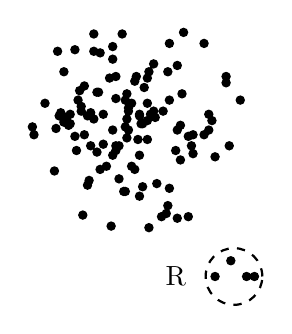
\begin{tikzpicture}[thick,scale=2, every node/.style={scale=5}]
	\fill (1.21, 0.56)  circle (0.3mm) (0.51, 1.02)  circle (0.3mm) (0.61, 1.44)  circle (0.3mm) (0.91, 1.54)  circle (0.3mm) (0.69, 0.58)  circle (0.3mm) (1.2, 1.3)  circle (0.3mm) (1.28, 0.96)  circle (0.3mm) (0.67, 1.21)  circle (0.3mm) (0.34, 0.95)  circle (0.3mm) (0.89, 0.83)  circle (0.3mm) (1.33, 0.38)  circle (0.3mm) (1.3, 1.55)  circle (0.3mm) (1.07, 0.99)  circle (0.3mm) (0.89, 0.62)  circle (0.3mm) (1.07, 0.87)  circle (0.3mm) (0.48, 0.67)  circle (0.3mm) (0.35, 0.9)  circle (0.3mm) (1.26, 1.34)  circle (0.3mm) (0.73, 1.54)  circle (0.3mm) (0.76, 1.17)  circle (0.3mm) (1.02, 1.03)  circle (0.3mm) (1.28, 0.74)  circle (0.3mm) (0.54, 1.3)  circle (0.3mm) (0.73, 1.43)  circle (0.3mm) (0.77, 1.42)  circle (0.3mm) (0.85, 0.93)  circle (0.3mm) (0.97, 1.1)  circle (0.3mm) (1.08, 1.3)  circle (0.3mm) (0.5, 1.43)  circle (0.3mm) (1.25, 0.8)  circle (0.3mm) (1.59, 0.83)  circle (0.3mm) (1.02, 0.51)  circle (0.3mm) (0.79, 0.84)  circle (0.3mm) (1.11, 1.05)  circle (0.3mm) (1.2, 0.45)  circle (0.3mm) (1.66, 1.12)  circle (0.3mm) (0.66, 0.39)  circle (0.3mm) (1.57, 1.27)  circle (0.3mm) (1.19, 0.4)  circle (0.3mm) (0.84, 0.32)  circle (0.3mm) (1.36, 0.9)  circle (0.3mm) (1.21, 1.48)  circle (0.3mm) (1.04, 0.57)  circle (0.3mm) (0.87, 0.83)  circle (0.3mm) (0.92, 0.54)  circle (0.3mm) (0.85, 1.46)  circle (0.3mm) (1.16, 0.38)  circle (0.3mm) (0.94, 0.88)  circle (0.3mm) (1.13, 0.59)  circle (0.3mm) (0.71, 0.83)  circle (0.3mm) (1.26, 0.37)  circle (0.3mm) (1.07, 0.87)  circle (0.3mm) (1.57, 1.23)  circle (0.3mm) (0.62, 0.8)  circle (0.3mm) (1.5, 0.76)  circle (0.3mm) (0.42, 1.1)  circle (0.3mm) (1.43, 1.48)  circle (0.3mm) (1.43, 0.9)  circle (0.3mm) (0.49, 0.94)  circle (0.3mm) (1.08, 0.31)  circle (0.3mm) 

(1.04, 0.97)  circle (0.3mm) (0.95, 0.93)  circle (0.3mm) (1.05, 1.2)  circle (0.3mm) (0.54, 0.98)  circle (0.3mm) (0.71, 1.04)  circle (0.3mm) (0.75, 1.17)  circle (0.3mm) (1.07, 1.26)  circle (0.3mm) (0.63, 1.12)  circle (0.3mm) (0.65, 1.08)  circle (0.3mm) (0.95, 1.05)  circle (0.3mm) (0.83, 1.26)  circle (0.3mm) (0.77, 0.68)  circle (0.3mm) (1.02, 0.77)  circle (0.3mm) (0.64, 1.18)  circle (0.3mm) (0.99, 0.68)  circle (0.3mm) (1.21, 1.12)  circle (0.3mm) (0.75, 0.79)  circle (0.3mm) (1.17, 1.05)  circle (0.3mm) (1.01, 0.87)  circle (0.3mm) (0.69, 1.02)  circle (0.3mm) (1.46, 0.93)  circle (0.3mm) (1.02, 1.02)  circle (0.3mm) (1.26, 0.93)  circle (0.3mm) (1.12, 1.01)  circle (0.3mm) (1.46, 1.03)  circle (0.3mm) (0.93, 0.95)  circle (0.3mm) (0.67, 0.9)  circle (0.3mm) (1.0, 1.27)  circle (0.3mm) (0.99, 1.24)  circle (0.3mm) (0.81, 0.7)  circle (0.3mm) (0.93, 0.54)  circle (0.3mm) (0.97, 0.7)  circle (0.3mm) (0.57, 0.96)  circle (0.3mm) (0.55, 1.01)  circle (0.3mm) (1.33, 0.89)  circle (0.3mm) (0.87, 0.8)  circle (0.3mm) (1.11, 1.35)  circle (0.3mm) (0.85, 1.38)  circle (0.3mm) (0.52, 1.04)  circle (0.3mm) (0.7, 0.61)  circle (0.3mm) (1.48, 0.99)  circle (0.3mm) (1.03, 0.97)  circle (0.3mm) (1.07, 1.1)  circle (0.3mm) (0.65, 1.05)  circle (0.3mm) (0.73, 1.0)  circle (0.3mm) (0.87, 1.13)  circle (0.3mm) (0.87, 1.27)  circle (0.3mm) (1.29, 1.16)  circle (0.3mm) (0.79, 1.03)  circle (0.3mm) (0.94, 1.0)  circle (0.3mm) (0.61, 0.89)  circle (0.3mm) (1.35, 0.83)  circle (0.3mm) (1.36, 0.78)  circle (0.3mm) (0.94, 1.16)  circle (0.3mm) (1.09, 1.03)  circle (0.3mm) (0.85, 0.77)  circle (0.3mm) (0.58, 1.03)  circle (0.3mm) (0.95, 1.07)  circle (0.3mm) (0.58, 0.97)  circle (0.3mm) (0.93, 1.12)  circle (0.3mm);


\draw[dashed] (1.62,0) circle (1.8mm); 
\fill (1.7,0)  circle (0.3mm) (1.75,0)  circle (0.3mm) (1.5,0)  circle (0.3mm) (1.6,0.1)  circle (0.3mm);
\node[scale = 0.2] at (1.25,0)    { R};

\end{tikzpicture}};
\end{frame}

%

\begin{frame}
	\frametitle{Outlier Detection (3): Clustering-Based Methods}
	Normal data belong to large and dense clusters, whereas outliers belong to\\ \blue{small or sparse clusters}, or do not belong to any cluster.
	\begin{itemize}
		
	\item \textbf{Example (right figure): two clusters}
	\begin{itemize}
		\item All points not in R form a large cluster
		\item The two points in R form a tiny cluster, thus are outliers.

	\end{itemize}
	\item \textbf{Many clustering methods}
	\begin{itemize}
		\item Thus also many clustering-based outlier detection methods
	\end{itemize}
	\item \textbf{Clustering is expensive.}
	\begin{itemize}
		\item Straightforward adaptation of a clustering method for outlier detection can be costly and does not scale up well for large data sets.
	\end{itemize}
	\end{itemize}
	
	\tikzoverlay at (12cm,6cm) {
	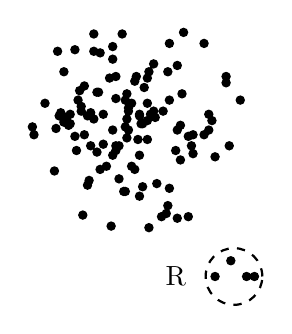
\begin{tikzpicture}[thick,scale=2, every node/.style={scale=5}]
	\fill (1.21, 0.56)  circle (0.3mm) (0.51, 1.02)  circle (0.3mm) (0.61, 1.44)  circle (0.3mm) (0.91, 1.54)  circle (0.3mm) (0.69, 0.58)  circle (0.3mm) (1.2, 1.3)  circle (0.3mm) (1.28, 0.96)  circle (0.3mm) (0.67, 1.21)  circle (0.3mm) (0.34, 0.95)  circle (0.3mm) (0.89, 0.83)  circle (0.3mm) (1.33, 0.38)  circle (0.3mm) (1.3, 1.55)  circle (0.3mm) (1.07, 0.99)  circle (0.3mm) (0.89, 0.62)  circle (0.3mm) (1.07, 0.87)  circle (0.3mm) (0.48, 0.67)  circle (0.3mm) (0.35, 0.9)  circle (0.3mm) (1.26, 1.34)  circle (0.3mm) (0.73, 1.54)  circle (0.3mm) (0.76, 1.17)  circle (0.3mm) (1.02, 1.03)  circle (0.3mm) (1.28, 0.74)  circle (0.3mm) (0.54, 1.3)  circle (0.3mm) (0.73, 1.43)  circle (0.3mm) (0.77, 1.42)  circle (0.3mm) (0.85, 0.93)  circle (0.3mm) (0.97, 1.1)  circle (0.3mm) (1.08, 1.3)  circle (0.3mm) (0.5, 1.43)  circle (0.3mm) (1.25, 0.8)  circle (0.3mm) (1.59, 0.83)  circle (0.3mm) (1.02, 0.51)  circle (0.3mm) (0.79, 0.84)  circle (0.3mm) (1.11, 1.05)  circle (0.3mm) (1.2, 0.45)  circle (0.3mm) (1.66, 1.12)  circle (0.3mm) (0.66, 0.39)  circle (0.3mm) (1.57, 1.27)  circle (0.3mm) (1.19, 0.4)  circle (0.3mm) (0.84, 0.32)  circle (0.3mm) (1.36, 0.9)  circle (0.3mm) (1.21, 1.48)  circle (0.3mm) (1.04, 0.57)  circle (0.3mm) (0.87, 0.83)  circle (0.3mm) (0.92, 0.54)  circle (0.3mm) (0.85, 1.46)  circle (0.3mm) (1.16, 0.38)  circle (0.3mm) (0.94, 0.88)  circle (0.3mm) (1.13, 0.59)  circle (0.3mm) (0.71, 0.83)  circle (0.3mm) (1.26, 0.37)  circle (0.3mm) (1.07, 0.87)  circle (0.3mm) (1.57, 1.23)  circle (0.3mm) (0.62, 0.8)  circle (0.3mm) (1.5, 0.76)  circle (0.3mm) (0.42, 1.1)  circle (0.3mm) (1.43, 1.48)  circle (0.3mm) (1.43, 0.9)  circle (0.3mm) (0.49, 0.94)  circle (0.3mm) (1.08, 0.31)  circle (0.3mm) 

(1.04, 0.97)  circle (0.3mm) (0.95, 0.93)  circle (0.3mm) (1.05, 1.2)  circle (0.3mm) (0.54, 0.98)  circle (0.3mm) (0.71, 1.04)  circle (0.3mm) (0.75, 1.17)  circle (0.3mm) (1.07, 1.26)  circle (0.3mm) (0.63, 1.12)  circle (0.3mm) (0.65, 1.08)  circle (0.3mm) (0.95, 1.05)  circle (0.3mm) (0.83, 1.26)  circle (0.3mm) (0.77, 0.68)  circle (0.3mm) (1.02, 0.77)  circle (0.3mm) (0.64, 1.18)  circle (0.3mm) (0.99, 0.68)  circle (0.3mm) (1.21, 1.12)  circle (0.3mm) (0.75, 0.79)  circle (0.3mm) (1.17, 1.05)  circle (0.3mm) (1.01, 0.87)  circle (0.3mm) (0.69, 1.02)  circle (0.3mm) (1.46, 0.93)  circle (0.3mm) (1.02, 1.02)  circle (0.3mm) (1.26, 0.93)  circle (0.3mm) (1.12, 1.01)  circle (0.3mm) (1.46, 1.03)  circle (0.3mm) (0.93, 0.95)  circle (0.3mm) (0.67, 0.9)  circle (0.3mm) (1.0, 1.27)  circle (0.3mm) (0.99, 1.24)  circle (0.3mm) (0.81, 0.7)  circle (0.3mm) (0.93, 0.54)  circle (0.3mm) (0.97, 0.7)  circle (0.3mm) (0.57, 0.96)  circle (0.3mm) (0.55, 1.01)  circle (0.3mm) (1.33, 0.89)  circle (0.3mm) (0.87, 0.8)  circle (0.3mm) (1.11, 1.35)  circle (0.3mm) (0.85, 1.38)  circle (0.3mm) (0.52, 1.04)  circle (0.3mm) (0.7, 0.61)  circle (0.3mm) (1.48, 0.99)  circle (0.3mm) (1.03, 0.97)  circle (0.3mm) (1.07, 1.1)  circle (0.3mm) (0.65, 1.05)  circle (0.3mm) (0.73, 1.0)  circle (0.3mm) (0.87, 1.13)  circle (0.3mm) (0.87, 1.27)  circle (0.3mm) (1.29, 1.16)  circle (0.3mm) (0.79, 1.03)  circle (0.3mm) (0.94, 1.0)  circle (0.3mm) (0.61, 0.89)  circle (0.3mm) (1.35, 0.83)  circle (0.3mm) (1.36, 0.78)  circle (0.3mm) (0.94, 1.16)  circle (0.3mm) (1.09, 1.03)  circle (0.3mm) (0.85, 0.77)  circle (0.3mm) (0.58, 1.03)  circle (0.3mm) (0.95, 1.07)  circle (0.3mm) (0.58, 0.97)  circle (0.3mm) (0.93, 1.12)  circle (0.3mm);


\draw[dashed] (1.62,0) circle (1.8mm); 
\fill (1.7,0)  circle (0.3mm) (1.75,0)  circle (0.3mm) (1.5,0)  circle (0.3mm) (1.6,0.1)  circle (0.3mm);
\node[scale = 0.2] at (1.25,0)    { R};

\end{tikzpicture}};	
\end{frame}

%

 \begin{frame}{Chapter: 8 Outlier Analysis}
\bf
    \begin{itemize}
        \item Outlier and Outlier Analysis
        \item  Outlier-Detection Methods
        \item \alert{Statistical Approaches}
        \item Proximity-Based Approaches
        \item Summary
    \end{itemize}
\end{frame}

%

\begin{frame}
	\frametitle{Statistical Approaches}
	Assume that the objects in a data set are \blue{generated by a stochastic process} (a generative model).
	\begin{itemize}
	\item \textbf{Idea:}
	\begin{itemize}
		\item Learn a generative model fitting the given data set, and then identify the objects in low-probability regions of the model as outliers.
	\end{itemize}
	\item \textbf{Methods divided into two categories:}
	\begin{itemize}
		\item Parametric vs. non-parametric
	\end{itemize}
	\item \textbf{Parametric method}
	\begin{itemize}
		\item Assumes that the normal data is generated by a parametric distribution with parameter \textbf{\alert{$\theta$}}.
		\item The probability density function of the parametric distribution \textbf{\alert{$f(x, \theta)$}} gives the probability that object \alert{$x$} is generated by the distribution.
		\item The smaller this value, the more likely $x$ is an outlier.
	\end{itemize}
	\end{itemize}
	
\end{frame}

%

\begin{frame}
  \frametitle{Statistical Approaches (2)}
  \begin{itemize}
    \item Non-parametric method
          \begin{itemize}
            \item Do not assume an a-priori statistical model
                  and determine the model from the input data.
            \item Not completely parameter-free,
                  but consider number and nature of the parameters to be flexible and not fixed in advance.
            \item Examples: \blue{histogram} and kernel-density estimation
          \end{itemize}
  \end{itemize}
\end{frame}

%

\begin{frame}
	\frametitle{Parametric Methods I: Detection of Univariate Outliers Based on Normal Distribution}
	\begin{itemize}
		\item Univariate data:
		      \begin{itemize}
		      	\item A data set involving only one attribute or variable
		      \end{itemize}
		\item Assumption:
		      \begin{itemize}
		      	\item Data are generated from a normal distribution
		      \end{itemize}
		\item Learn the parameters from the input data, and identify the points with low probability as outliers.
		      \begin{itemize}
		      	\item Use the \blue{maximum-likelihood method} to estimate $\mu$ and $\sigma$:
		      	$$
		      	ln\mathcal{L}(\mu, \sigma^2)= 
		      	\frac1n \sum_{i=1}^n \ln f(x_i \mid \sigma^2), = 
		      	-\frac{n}{2}ln(2\pi)-\frac{n}{2}ln \sigma^2 - \frac{1}{2 \sigma^2} \sum_{i=1}^n(x_i - \mu)^2 
		      	$$
		      	\item Taking derivatives with respect to $\mu$ and $\sigma^2$, we derive the following maximum-likelihood estimates:
		      	
				 \qquad \qquad$\widehat{\mu}=\overline{x}= \frac{1}{n} \sum_{i=1}^n x_i$ \qquad $\widehat{\sigma^2} = \frac{1}{n} \sum_{i=1}^n (x_i-\overline{x})^2$ 
		      	
		      	
		      \end{itemize}
	\end{itemize}
\end{frame}

%

\begin{frame}
	\frametitle{Parametric Methods I: Detection of Univariate Outliers Based on Normal Distribution (2)}
	\begin{itemize}
		\item Example
		      \begin{itemize}
		      	\item Average temperature: {24.0, 28.9, 28.9, 29.0, 29.1, 29.1, 29.2, 29.2, 29.3, 29.4}
		      	\item For these data with n = 10, we have \\
		      	\qquad \qquad \qquad $\widehat{\mu}=28.61$ \qquad \qquad $\widehat{\sigma}=\sqrt{2.29}=1.51$ 
		      	\item Then the most deviating value 24.0 is 4.61 away form the estimated mean.
		      	\item $\mu \pm 3\sigma $ contains 99.7\% of the data under the assumption of normal distribution.
		      	\item Because 4.61 / 1.51  =  3.04  >  3, the probability that 24.0 is generated by a normal distribution is less than 0.15\%.
		      	      \begin{itemize}
		      	      	\item Each "tail" to the left and to the right of the 99.7\% has 0.15\%.
		      	      \end{itemize}
		      	\item Hence, 24.0 identified as an outlier.
		      \end{itemize}
	\end{itemize}
\end{frame}

%

\begin{frame}
	\frametitle{Parametric Methods I: The Grubb's Test}
	\begin{itemize}
		\item Univariate outlier detection: The Grubb's test (maximum normed residual test)
		      \begin{itemize}
		      	\item Another statistical method under normal distribution
		      	\item For each object \textbf{\alert{x}} in a data set, compute its \blue{z-score}:  $\textbf{\alert{z}} = | x - x_m | / s$
		      	      \begin{itemize}
		      	      	\item where \textbf{\alert{$x_m$}} is the mean and \textbf{\alert{s}} the standard deviation of the input data.
		      	      \end{itemize}
		      	\item x is an outlier, if
		      \end{itemize}
		$$ z \geq \frac{N-1}{\sqrt{N}} \sqrt{\frac{t^2_{\alpha/(2N),N-2}}{N-2 + t^2_{\alpha/(2N),N-2}}} $$
		      \begin{itemize}
		      	\item where $t^2_{\alpha/(2N),N-2}$is the value taken by a t-distribution at a significance level of $\alpha / (2N)$, and N is the \# of objects in the data set.
		      \end{itemize}
	\end{itemize}
\end{frame}

%

\begin{frame}
	\frametitle{Parametric Methods II: Detection of Multivariate Outliers}
	\begin{itemize}
		\item \textbf{Multivariate data}:
		      \begin{itemize}
		      	\item A data set involving \blue{two or more attributes} or variables
		      \end{itemize}
		\item \textbf{Transform the multivariate outlier-detection task into a univariate outlier-detection problem.}
		\item \textbf{Method 1. Compute Mahalanobis distance}
		      \begin{itemize}
		      	\item Let \textbf{\alert{ō}} be the mean vector for a multivariate data set. Mahalanobis distance for an object \textbf{\alert{o}} to \textbf{ō} is $\alert{MDist(\textbf{o}, \textbf{ō})} = (\textbf{o} - \textbf{ō})^T S-1 (\textbf{o} - \textbf{ō})$ where $S$ is the covariance matrix.
		      	\item Use the Grubb's test on this measure to detect outliers.
		      \end{itemize}
		\item \textbf{Method 2. Use $\chi^2$ statistic}
		      \begin{itemize}
		      	 \item $$\chi^2 = \sum^n_{i=1} \frac{(o_i-E_i)^2}{E_i} $$
		      	\item where $E_i$ is the mean of the i-dimension among all objects, and \textbf{\alert{n}} is the dimensionality.
		      	\item If $\chi^2$ 2 statistic is large, then object \textbf{$o_i$} is an outlier.
		      \end{itemize}
	\end{itemize}
\end{frame}

%

\begin{frame}
	\frametitle{Parametric Methods III: Using Mixture of Parametric Distributions}
	\begin{itemize}
		\item \textbf{Assuming that data are generated by a normal distribution could sometimes be overly simplified.}
		\item \textbf{Example (right figure):}
		      \begin{itemize}
		      	\item The objects between the two clusters cannot be captured as outliers since they are close to the estimated mean.
		      \end{itemize}
		\item \textbf{Assume the normal data is generated by \blue{two normal distributions.}}
		      \begin{itemize}
		      	\item For any object \textbf{\alert{o}} in the data set, the probability that o is generated by the mixture of the two distributions is given by
		      	\item $$Pr(o|\Theta_1, \Theta_2) = f_{\Theta_1}(o) + f_{\Theta_2}(o)$$
		      	
		      	      \begin{itemize}
		      	      	\item where $f_{\theta 1}$ and $f_{\theta 2}$ are the probability density functions of $\theta_1$ and $\theta_2$.
		      	      \end{itemize}
		      	\item Then use expectation-maximization (EM) algorithm to learn the parameters $\mu_1, \sigma_1, \mu_2, \sigma_2$ from the data.
		      	\item An object \textbf{o} is an outlier if it does not belong to any cluster.
		      \end{itemize}
	\end{itemize}
\end{frame}

%

\begin{frame}
	\frametitle{Non-Parametric Methods:Detection Using Histogram}
	\begin{itemize}
		\item \textbf{The model of normal data is learned from the input data without any apriori structure.}
		      \begin{itemize}
		      	\item Often makes fewer assumptions about the data, and thus can be applicable in more scenarios.
		      \end{itemize}
		\item \textbf{Outlier detection using histogram:}
		      \begin{itemize}
		      	\item Figure shows the histogram of purchase amounts in transactions.
		      	\item A transaction with the amount of \$7,500is an outlier, since only 0.2
\% of the transactions have an amount higher than \$5,000.
		      \end{itemize}
	\end{itemize}
	\includegraphics[width=0.3\textwidth]{img/histogram8.png}

\end{frame}

%

\begin{frame}
	\frametitle{Non-Parametric Methods:Detection Using Histogram (2)}
	\begin{itemize}
		\item Problem:
		      \begin{itemize}
		      	\item Hard to \blue{choose an appropriate bin size} for histogram
		      	      \begin{itemize}
		      	      	\item Too small bin size $\rightarrow$ normal objects in empty/rare bins, false positive
		      	      	\item Too big bin size $\rightarrow$ outliers in some frequent bins, false negative
		      	      \end{itemize}
		      \end{itemize}
		\item Solution:
		      \begin{itemize}
		      	\item Adopt kernel-density estimation to estimate the probability-density distribution of the data.
		      	      \begin{itemize}
		      	      	\item If the estimated density function is high, the object is likely normal.
		      	      	\item Otherwise, it is likely an outlier.
		      	      \end{itemize}
		      \end{itemize}
	\end{itemize}
\end{frame}

%

\begin{frame}
	\frametitle{Chapter 8: Outlier Analysis}
	\begin{itemize}
		\item Outlier and Outlier Analysis
		\item Outlier-Detection Methods
		\item Statistical Approaches
		\item \alert{Proximity-Based Approaches}
		\item Summary
	\end{itemize}
\end{frame}

%

\begin{frame}
	\frametitle{Proximity-Based Approaches:Distance-Based vs. Density-Based Outlier Detection}
	\begin{itemize}
		\item \textbf{Intuition:}
		      \begin{itemize}
		      	\item Objects that are \blue{far away from the others} are outliers.
		      \end{itemize}
		\item \textbf{Assumption of proximity-based approach:}
		      \begin{itemize}
		      	\item The proximity of an outlier deviates significantly from that of most of the others in the data set.
		      \end{itemize}
		\item \textbf{Two types of proximity-based outlier-detection methods}
		      \begin{itemize}
		      	\item \blue{Distance-based} outlier detection:
		      	      \begin{itemize}
		      	      	\item An object \textbf{o} is an outlier, if its neighborhood does not have enough other points.
		      	      \end{itemize}
		      	\item \blue{Density-based} outlier detection:
		      	      \begin{itemize}
		      	      	\item An object \textbf{o} is an outlier, if its density is relatively much lower than that of its neighbors.
		      	      \end{itemize}
		      \end{itemize}
	\end{itemize}
\end{frame}

%
\begin{frame}
\frametitle{Distance-Based Outlier Detection }
	\begin{itemize}
		\item For each object \textbf{o}, examine the \# of other objects in the \blue{r-neighborhood} of \textbf{o}, where \alert{\textbf{r}} is a user-specified \textbf{distance threshold}.
		\item An object \textbf{o} is an outlier if most (taking \alert{$\pi$} as a \textbf{fraction threshold}) of the objects in \alert{\textbf{D}} are far away from o, i.e., not in the r-neighborhood of \textbf{o}
	\end{itemize}
	
	\begin{itemize}
		\item \textbf{An object o is a \alert{DB(r, $\pi$) outlier} if}
		\begin{itemize}		
		\item $$\frac{||\{o'|dist(o,o')\leq r \}|| }{||D||} \leq \pi $$
		\item Equivalently, one can check the distance between \textbf{o} and its $k$-th nearest neighbor \alert{\textbf{$o_k$}}, where $k=\lceil \pi ||D||\rceil$                       . \\
		\item \textbf{o} is an outlier, if $dist(\textbf{o}, \textbf{o}_k)$ > r
	
		\end{itemize}		
		
	\end{itemize}

\end{frame}

%

\begin{frame}
	\frametitle{Distance-Based Outlier Detection (2)}
	\begin{itemize}
		\item \textbf{Efficient computation: \blue{Nested-loop algorithm}}
		      \begin{itemize}
		      	\item For any object \textbf{$o_i$}, calculate its distance from other objects, and count the \# of other objects in the r-neighborhood.
		      	\item If $\pi n $ other objects are within r distance, terminate the inner loop.
		      	\item Otherwise, \textbf{$o_i$} is a DB(r, $\pi$) outlier.
		      \end{itemize}
		\item \textbf{Efficiency:}
		      \begin{itemize}
		      	\item Actually, CPU time is not O($n^2$) but linear to the data set size, since for most non-outlier objects, the inner loop terminates early.
		      \end{itemize}
	\end{itemize}
\end{frame}

%

\begin{frame}
	\frametitle{Distance-Based Outlier Detection (3)}
	\begin{itemize}
		\item Why is efficiency still a concern?
		      \begin{itemize}
		      	\item If the complete set of objects cannot be held in main memory, there is significant cost for I/O swapping.
		      \end{itemize}
		\item The major cost:
		      \begin{itemize}
		      	\item (1)  Each object is tested against the whole data set\\
		      	why not only against its close neighbors?
		      	\item (2)  Objects are checked one by one\\		      	
		      	why not group by group?
		      \end{itemize}
	\end{itemize}
\end{frame}

%

\begin{frame}
	\frametitle{Distance-Based Outlier Detection:A Grid-Based Method}
	\begin{itemize}
		\item \textbf{CELL:}
		      \begin{itemize}
		      	\item Data space is partitioned into a multi-D grid.
		      	\item Each cell is a hyper cube with diagonal length $r/2$.
		      	      \begin{itemize}
		      	      	\item \alert{\textbf{r}} distance threshold parameter
		      	      	\item \alert{\textbf{l}} dimensions: edge of each cell $r / (2\sqrt{l})$ long
		      	      \end{itemize}
		      \end{itemize}
		\item \textbf{Level-1 cells:}
		      \begin{itemize}
		      	\item Immediately next to cell \alert{\textbf{C}}
		      	\item For any possible point \alert{\textbf{x}} in C and\\ any possible point \alert{\textbf{y}} in a level-1 cell: $dist(x,y) \leq r$
		      \end{itemize}
		\item \textbf{Level-2 cells:}
		      \begin{itemize}
		      	\item One or two cells away from C
		      	\item For any possible point x  in cell C and\\ any point y such that $dist(x,y) \geq r$, y is in a level-2 cell.
		      	\item 
		      \end{itemize}
	\end{itemize}
	\tikzoverlay at (10cm,5cm) {\includegraphics[width=0.3\textwidth]{img/grid8.png}};
\end{frame}


\begin{frame}
	\frametitle{Distance-Based Outlier Detection: A Grid-Based Method (2)}
	\begin{itemize}
		\item Total number of objects in cell C: \alert{a}
		\item Total number of objects in level-1 cells: \alert{b1}
		\item Total number of objects in level-2 cells: \alert{b2}
	\end{itemize}
	%need item	
	\textbf{Level-1 cell pruning rule}:
	\begin{itemize}
		\item if $a + b1 > \lceil \pi n \rceil$, then every object o in C is not a DB(r, $\pi$) outlier, because all objects in C and the level-1 cells are in the r-neighborhood of o,and there are at least $\lceil \pi n \rceil$ such objects.
	\end{itemize}
	% need item
	 \textbf{Level-2 cell pruning rule:}
	\begin{itemize}
		\item if $ a + b1 + b2 < \lceil \pi n \rceil + 1,$then all objects in C are $DB(r, \pi)$  outliers, because all of their r-neighborhoods have less than $\lceil \pi n\rceil$ other objects.
	\end{itemize}
	%need item
	\textbf{Only need to check the objects that cannot be pruned}
	\begin{itemize}
		\item Even for such an object o, only need to compute the distance between o and the objects in level-2 cells
		      \begin{itemize}
		      	\item Since beyond level-2, distance from o is more than r
		      \end{itemize}
	\end{itemize}
\end{frame}



\begin{frame}
	\frametitle{Density-Based Outlier Detection}
	\begin{itemize}
		\item \blue{Local outliers}:
		      \begin{itemize}
		      	\item Outliers compared to their local neighborhoods, not to global data distribution
		      	      \begin{itemize}
		      	      	\item In Fig., O1 and O2 are local outliers to C1, O3 is a global outlier, but O4 is not an outlier.
		      	      	\item However, distance of O1 and O2 to objects in dense cluster C1 is smaller than average distance in sparse cluster C2.
		      	      	\item Hence, O1 and O2 are not distance-based outliers.
		      	      \end{itemize}
		      \end{itemize}
		\item Intuition:
		      \begin{itemize}
		      	\item Density around \blue{outlier} object \blue{significantly different}\\ from density around its neighbors.
		      \end{itemize}
	\end{itemize}
	\tikzoverlay at (9.5cm,2cm) {
	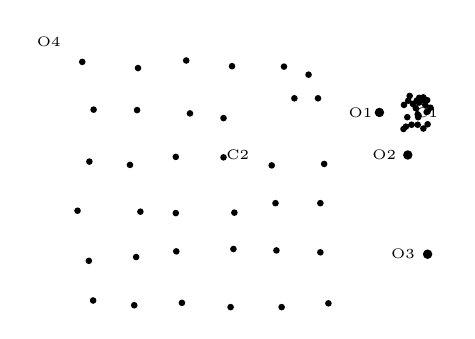
\begin{tikzpicture}[thick,scale=0.6, every node/.style={scale=5}]
\fill (0.14, 0.02)  circle (0.7mm) (0.05, 0.86)  circle (0.7mm) (-0.19, 1.92)  circle (0.7mm) (0.06, 2.96)  circle (0.7mm) (0.15, 4.06)  circle (0.7mm) (-0.09, 5.07)  circle (0.7mm) (1.01, -0.08)  circle (0.7mm) (1.05, 0.94)  circle (0.7mm) (1.14, 1.9)  circle (0.7mm) (0.92, 2.89)  circle (0.7mm) (1.07, 4.05)  circle (0.7mm) (1.09, 4.94)  circle (0.7mm) (2.02, -0.03)  circle (0.7mm) (1.9, 1.06)  circle (0.7mm) (1.89, 1.87)  circle (0.7mm) (1.89, 3.06)  circle (0.7mm) (2.19, 3.98)  circle (0.7mm) (2.11, 5.1)  circle (0.7mm) (3.05, -0.12)  circle (0.7mm) (3.11, 1.11)  circle (0.7mm) (3.13, 1.88)  circle (0.7mm) (2.9, 3.05)  circle (0.7mm) (2.9, 3.88)  circle (0.7mm) (3.08, 4.98)  circle (0.7mm) (4.13, -0.12)  circle (0.7mm) (4.02, 1.08)  circle (0.7mm) (4.0, 2.08)  circle (0.7mm) (3.92, 2.88)  circle (0.7mm) (4.4, 4.3)  circle (0.7mm) (4.18, 4.97)  circle (0.7mm) (5.12, -0.04)  circle (0.7mm) (4.95, 1.04)  circle (0.7mm) (4.95, 2.08)  circle (0.7mm) (5.03, 2.91)  circle (0.7mm) (4.9, 4.3)  circle (0.7mm) (4.7, 4.8)  circle (0.7mm) ; 

%cluster
\fill (7.22, 4.02)  circle (0.7mm) (7.01, 3.74)  circle (0.7mm) (7.17, 4.16)  circle (0.7mm) (7.04, 4.31)  circle (0.7mm) (7.28, 4.1)  circle (0.7mm) (7.22, 3.75)  circle (0.7mm) (6.99, 4.25)  circle (0.7mm) (7.13, 3.66)  circle (0.7mm) (7.03, 3.93)  circle (0.7mm) (6.84, 4.35)  circle (0.7mm) (6.72, 4.16)  circle (0.7mm) (7.14, 4.27)  circle (0.7mm) (6.88, 3.74)  circle (0.7mm) (7.04, 4.21)  circle (0.7mm) (6.79, 3.9)  circle (0.7mm) (7.01, 3.96)  circle (0.7mm) (7.13, 4.32)  circle (0.7mm) (6.71, 3.65)  circle (0.7mm) (6.76, 3.7)  circle (0.7mm) (7.21, 4.26)  circle (0.7mm) (7.02, 3.9)  circle (0.7mm) (7.2, 4.01)  circle (0.7mm) (6.91, 4.18)  circle (0.7mm) (6.81, 4.25)  circle (0.7mm) (6.97, 4.09)  circle (0.7mm);

%outlier O3
\fill (7.22, 1)  circle (1mm);
\node[scale = 0.2] at (6.7, 1)    {\tiny O3};

%O1
\fill (6.2, 4)  circle (1mm);
\node[scale = 0.2] at (5.8, 4)    {\tiny O1};

%O2
\fill (6.8, 3.1)  circle (1mm);
\node[scale = 0.2] at (6.3, 3.1)    {\tiny O2};


\node[scale = 0.2] at (7.2, 4)    {\tiny C1};
\node[scale = 0.2] at (3.2, 3.1)    {\tiny C2};
\node[scale = 0.2] at (-0.8, 5.5)    {\tiny O4};
\end{tikzpicture}};
\end{frame}

\begin{frame}
	\frametitle{Density-Based Outlier Detection (2)}
		
	\begin{itemize}
		\item Method:
		      \begin{itemize}
		      	\item Use the \blue{relative density} of an object against its neighbors as the indicator of the degree of the object being outliers
		      \end{itemize}
	\end{itemize}
	 \textbf{\alert{k-distance} of an object \textbf{\alert{o}}}
	\begin{itemize}
		\item $dist_k(\textbf{o})$
		\item distance $dist(\textbf{o, p})$ between o and its k-nearest neighbour \alert{p}
		      \begin{itemize}
		      \item test
		      	\item at least $k$ objects $\textbf{o'} \in D - {\textbf{o}}$ such that $dist(\textbf{o, o'}) \leq dist(\textbf{o, p})$
		      	\item at most $k - 1$ objects $\textbf{o''} \in D - {\textbf{o}}$ such that $dist(\textbf{o}, \textbf{o'}) > dist(\textbf{o, p})$
		      \end{itemize}
		\item \alert{k-distance neighborhood of \textbf{o}}:
		      \begin{itemize}
		      	\item $N_k(\textbf{o}) = {\textbf{\textbf{o'}} | \textbf{o'} \in D, dist(\textbf{o}, \textbf{o'}) \leq distk(\textbf{o})}$
		      	\item $N_k(\textbf{o})$ could be bigger than k since multiple objects may have identical distance to $\textbf{o}$
		      \end{itemize}
	\end{itemize}
\end{frame}




\begin{frame}
	\frametitle{Local Outlier Factor}
	\begin{itemize}
		\item \alert{Reachability distance from $o'$ to $o$:}\\
		       $reachdist_k(o' \leftarrow o) = max\{dist_k(o),dist(o,o')\}$
		      \begin{itemize}
		      	\item where k is a user-specified parameter
		      \end{itemize}
		\item \alert{Local reachability density of $o$:}\\
		$ldr_k(o) = \frac{||N_k(o)||}{\sum_{o' \in N_k(o)}reachdist_k(o' \leftarrow o)}$
		\item \alert{LOF (Local Outlier Factor) of $o$:}
		      \begin{itemize}
		      	\item The average of the ratio of local reachability of $o$ and those of $o$'s k-nearest neighbors
		      \end{itemize}
		$ LOF_k(o)=\frac{\sum_{o' \in N_k(o)}\frac{lrd_k(o')}{lrd_k(o)} }{||N_k(o)||} =
		    \sum_{o' \in N_k(o)}lrd_k(o') * \sum_{o' \in N_k(o)}reachdist_k(o' \leftarrow o)
		$
		      \begin{itemize}
		      	\item 
		      	\item The lower the local reachability density of $o$, and the higher the local reachability density of the kNN of $o$, the higher LOF
		      	\item This captures a local outlier whose local density is relatively low comparing to the local densities of its kNN.
		      \end{itemize}
	\end{itemize}
	
	\tikzoverlay at (9cm,7.5cm){\includegraphics[width=0.35\textwidth]{img/density.png}};
\end{frame}

%

\begin{frame}
	\frametitle{Chapter 8: Outlier Analysis}
	\begin{itemize}
		\item Outlier and Outlier Analysis
		\item Outlier-Detection Methods
		\item Statistical Approaches
		\item Proximity-Based Approaches
		\item \alert{Summary}
	\end{itemize}
\end{frame}

%

\begin{frame}
	\frametitle{Summary}
	\begin{itemize}
		\item  \textbf{Types of outliers}
		      \begin{itemize}
		      	\item Global, contextual \& collective outliers
		      \end{itemize}
		\item \textbf{Outlier detection}
		      \begin{itemize}
		      	\item Supervised, semi-supervised, or unsupervised
		      \end{itemize}
		\item \textbf{Statistical (or model-based) approaches}
		\item \textbf{Proximity-based approaches}
		\item \textbf{Not covered here:}
		      \begin{itemize}
		      	\item Clustering-based approaches
		      	\item Classification approaches
		      	\item Mining contextual and collective outliers
		      	\item Outlier detection in high dimensional data
		      \end{itemize}
	\end{itemize}
\end{frame}

  
  { % Questions?
    \setbeamertemplate{footline}[frame number]
    \begin{frame}[c]
      \begin{center}
        Thank you for your attention.\\
        {\bf Any questions about the eighth chapter?}\\[0.5cm]
        Ask them now, or again, drop me a line: \\
        \faSendO \ \texttt{luciano.melodia@fau.de}.
      \end{center}
    \end{frame}
  }
  
  \begin{frame}
	\frametitle{References}
	\begin{itemize}
		\item B. Abraham and G.E.P. Box. Bayesian analysis of some outlier problems in time series. Biometrika, 66:229–248, 1979.
		\item M. Agyemang, K. Barker, and R. Alhajj. A comprehensive survey of numeric and symbolic outlier mining techniques. Intell. Data Anal., 10:521–538, 2006.
		\item F. J. Anscombe and I. Guttman. Rejection of outliers. Technometrics, 2:123–147, 1960.
		\item D. Agarwal. Detecting anomalies in cross-classified streams: a Bayesian approach. Knowl. Inf. Syst., 11:29–44, 2006.
		\item F. Angiulli and C. Pizzuti. Outlier mining in large high-dimensional data sets. TKDE, 2005.
		\item C.C. Aggarwal and P.S. Yu. Outlier detection for high dimensional data. SIGMOD'01.
		\item R.J. Beckman and R.D. Cook. Outlier...s. Technometrics, 25:119–149, 1983.
		\item I. Ben-Gal. Outlier detection. In: O. Maimon and L. Rockach (eds.), Data Mining and Knowledge Discovery Handbook: A Complete Guide for Practitioners and Researchers, Kluwer Academic, 2005.
	\end{itemize}
\end{frame}

\begin{frame}
	\frametitle{References (2)}
	\begin{itemize}
		\item M.M. Breunig, H.-P. Kriegel, R. Ng, and J. Sander. LOF: Identifying density-based local outliers. SIGMOD'00.
		\item D. Barbara, Y. Li, J. Couto, J.-L. Lin, and S. Jajodia. Bootstrapping a data mining intrusion detection system. SAC'03.
		\item Z.A. Bakar, R. Mohemad, A. Ahmad, and M. M. Deris. A comparative study for outlier detection techniques in data mining. IEEE Conf. on Cybernetics and Intelligent Systems, 2006.
		\item S. D. Bay and M. Schwabacher. Mining distance-based outliers in near linear time with randomization and a simple pruning rule. KDD'03.
		\item D. Barbara, N. Wu, and S. Jajodia. Detecting novel network intrusion using Bayesian estimators. SDM'01.
		\item V. Chandola, A. Banerjee, and V. Kumar. Anomaly detection: A survey. ACM Computing Surveys, 41:1–58, 2009.
		\item D. Dasgupta and N.S. Majumdar. Anomaly detection in multidimensional data using negative selection algorithm. CEC'02.
	\end{itemize}
\end{frame}

\begin{frame}
	\frametitle{References (3)}
	\begin{itemize}
		\item E. Eskin, A. Arnold, M. Prerau, L. Portnoy, and S. Stolfo. A geometric framework for unsupervised anomaly detection: Detecting intrusions in unlabeled data. Int. Conf. of Data Mining for Security Applications, 2002.
		\item E. Eskin. Anomaly detection over noisy data using learned probability distributions. ICML'00.
		\item T. Fawcett and F. Provost. Adaptive fraud detection. Data Mining and Knowledge Discovery, 1:291–316, 1997.
		\item V.J. Hodge and J. Austin. A survey of outlier detection methodologies. Artif. Intell. Rev., 22:85–126, 2004.
		\item D. M. Hawkins. Identification of Outliers. Chapman and Hall, London, 1980.
		\item Z. He, X. Xu, and S. Deng. Discovering cluster-based local outliers. Pattern Recogn. Lett., 24, June, 2003.
		\item W. Jin, K. H. Tung, and J. Han. Mining top-n local outliers in large databases. KDD'01.
	\end{itemize}
\end{frame}

\begin{frame}
	\frametitle{References (4)}
	\begin{itemize}
		\item W. Jin, A. K. H. Tung, J. Han, and W. Wang. Ranking outliers using symmetric neighborhood relationship. PAKDD'06.
		\item E. Knorr and R. Ng. A unified notion of outliers: Properties and computation. KDD'97.
		\item E. Knorr and R. Ng. Algorithms for mining distance-based outliers in large datasets. VLDB'98.
		\item E. M. Knorr, R. T. Ng, and V. Tucakov. Distance-based outliers: Algorithms and applications. VLDB J., 8:237–253, 2000.
		\item H.-P. Kriegel, M. Schubert, and A. Zimek. Angle-based outlier detection in high-dimensional data. KDD'08.
		\item M. Markou and S. Singh. Novelty detection: A review—part 1: Statistical approaches. Signal Process., 83:2481–2497, 2003.
		\item M. Markou and S. Singh. Novelty detection: A review—part 2: Neural network based approaches. Signal Process., 83:2499–2521, 2003.
		\item C. C. Noble and D. J. Cook. Graph-based anomaly detection. KDD'03.
	\end{itemize}
\end{frame}

\begin{frame}
	\frametitle{References (5)}
	\begin{itemize}
		\item S. Papadimitriou, H. Kitagawa, P.B. Gibbons, and C. Faloutsos. Loci: Fast outlier detection using the local correlation integral. ICDE'03.
		\item A. Patcha and J.-M. Park. An overview of anomaly detection techniques: Existing solutions and latest technological trends. Comput. Netw., 51, 2007.
		\item X. Song, M. Wu, C. Jermaine, and S. Ranka. Conditional anomaly detection. IEEE Trans. on Knowl. and Data Eng., 19, 2007.
		\item Y. Tao, X. Xiao, and S. Zhou. Mining distance-based outliers from large databases in any metric space. KDD'06.
		\item N. Ye and Q. Chen. An anomaly detection technique based on a chi-square statistic for detecting intrusions into information systems. Quality and 			Reliability Engineering International, 17:105–112, 2001.
		\item B.-K. Yi, N. Sidiropoulos, T. Johnson, H. V. Jagadish, C. Faloutsos, and A. Biliris. Online data mining for co-evolving time sequences. ICDE'00.
	\end{itemize}
\end{frame}

\end{document}
